\documentclass{article}

\usepackage[margin=0.5in]{geometry}
\usepackage[czech]{babel}
\usepackage{graphicx, amsmath}
\usepackage{booktabs, vwcol, multicol}
% \usepackage[texMathDollars,pipeTables=true,tableCaptions,hybrid]{markdown}

\begin{document}

\begin{center}
  \Large \bfseries
Modely konkurence
\end{center}
\pagestyle{empty}

\begin{multicols}2
Modely konkurence vychází z klasické logistické rovnice
$$    \frac{\mathrm dx}{\mathrm dt} = rx\left(1-\frac{x}{K}\right) $$
napsané samostatně pro každou z populací a doplněnou o skutečnost, že část nosné kapacity zaplní konkurující druh. 
Dvě konkurující si populace o velikostech $x$ a $y$ je možno modelovat dvojicí
rovnic
\begin{equation*}
  \begin{aligned}
    \frac{\mathrm dx}{\mathrm dt} &= r_1x\left(1-\frac{x+w_1y}{K_1}\right) \\
    \frac{\mathrm dy}{\mathrm dt} &= r_2y\left(1-\frac{y+w_2x}{K_2}\right), 
  \end{aligned}
\end{equation*}
kde $w_1$ a $w_2$ jsou koeficienty, vyjadřující, jak jedna populace zaplňuje nosnou kapacitu populace druhé. 
Zpravidla systém upravujeme rozdělením zlomkz na dva členy a roznásobením koeficientem před závorkou do tvaru
\begin{equation*}
  \begin{aligned}
    \frac{\mathrm dx}{\mathrm dt} &= x(a-bx-cy) \\
    \frac{\mathrm dy}{\mathrm dt} &= y(\alpha-\beta x - \gamma y), 
  \end{aligned}
\end{equation*}
kde $b$ a $\gamma$ jsou parametry vnitrodruhové konkurence a $c$ a $\beta$ parametry mezidruhové konkurence.

Počátek je vždy nestacionárním bodem. Pokud bude přítomno malé
množství obou druhů, budou oba druhy růst.

Model vykazuje tři druhy chování.
\begin{itemize}\itemsep -5 pt
\item Může dojít k dominanci jednoho z druhů. V tomto případě jedna
  populace vymírá a druhá konverguje k nosné kapacitě. Toto nastává,
  pokud pro jednu populaci je mezidruhová konkurence silnější než
  vnitrodruhová a pro druhou je tomu naopak.
\item V případě že obě mezidruhové konkurence jsou malé, dojde ke
  slabé konkurenci. Žádná z populací nevymírá, obě populace setrvávají
  na nenulových hodnotách.
\item V případě silné mezidruhové konkurence dochází k silné
  konkurenci, kdy jedna z populací vymírá a druhá konverguje ke své
  nosné kapacitě. Na rozdíl od dominance jednoho druhu v tomto případě
  výchozí stav rozhoduje o tom, která z populací přežívá a která
  vymírá.
\end{itemize}

Při posuzování síly konkurence nestačí posuzovat pouze koeficienty
$b$, $c$, $\beta$, $\gamma$, ale je nutno je posuzovat i s ohledem na
rychlosti růstu $a$ a $\alpha$. Například z první rovnice vidíme, že
nosná kapacita pro populaci $x$ bez přítomnosti populace $y$ je
$\frac ab$. Z druhé rovnice vidíme, že pokud je výraz
$$\alpha - \beta \frac ab$$ kladný, populace $y$ roste a pokud záporný,
populace $y$ klesá. V prvním případě je tedy bod odpovídající
přítomnosti jenom populace $x$ nestabilní, introdukce populace $y$
vede k rozšíření $y$ a proto se jedná buď o slabou konkurenci nebo
dominanci druhu $y$. Podobně znaménko výrazu $a-c\frac\alpha\gamma$
rozhoduje o tom, zda při introdukci populace $x$ do prostředí
obsazeného populací $y$ populace $x$ prosperuje či nikoliv a opět
odsud odvodíme, o který ze scénářů se může jednat.

\end{multicols}

\hbox to \hsize{\hss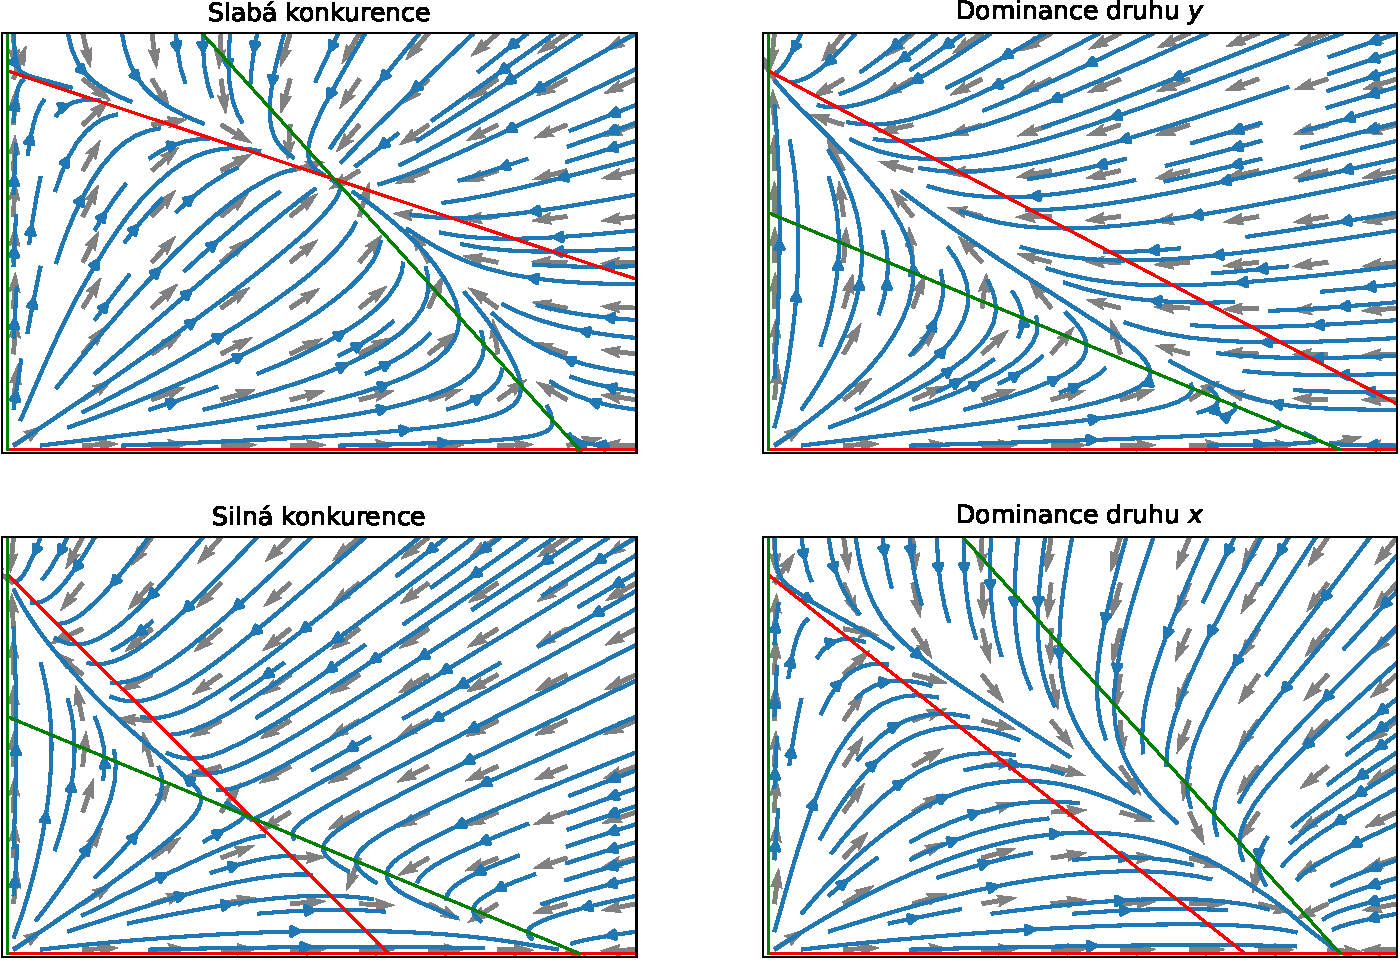
\includegraphics[width=0.9\linewidth]{img_konkurence.pdf}\hss}


\end{document}


%%% Local Variables: 
%%% TeX-command-extra-options: "-shell-escape"
%%% End:
